\section{The Identity-Transformation Approach of UPPRESSO}
\label{sec:challenge}

In this section, we analyze the challenges to design secure privacy-preserving SSO systems,
     and provide an overview of the identity-transformation approach proposed in UPRESSO.

\subsection{Security Requirements of SSO}
\label{subsec:basicrequirements}
We summarize the basic requirements of SSO systems based on existing theoretical analyses~\cite{ArmandoCCCT08,FettKS16, FettKS17} and practical attacks~\cite{SomorovskyMSKJ12,WangCW12,ArmandoCCCPS13,ZhouE14,WangZLLYLG15,WangZLG16,YangLLZH16,MainkaMS16,MohsenS16,MainkaMSW17,YangLCZ18,YangLS17,ShiWL19}. These requirements enable an SSO system to provide qualified authentication services for RPs,
    through identity proofs.
\begin{itemize}
\item
\textbf{User identification.} When a user logs into a certain RP for multiple times by submitting identity proofs,
 the RP extracts the identical user identifier from these identity proofs,
    to provide personalized services for this user.

\item
\textbf{RP designation.} The designated receiver (or RP) is specified in an identity proof,
    so that this identity proof is accepted by the visited RP only.

\item
\textbf{Integrity and confidentiality.}
 Only the IdP is trusted to generate identity proofs,
 RPs do not accept an identity proof with any modification or a forged one.
%RPs should only accept the valid identity proof.
Meanwhile, a valid identity proof is transmitted only to the user and the designated RP.
% confidentiality of the identity proof is ensured during the transmission among the IdP, user and the designated RP.
\end{itemize}



%These basic requirements are the minimum properties that an SSO system has to provide.
% therefore RPs should be able to identify the user with the help from IdP.
First of all,
    user identification is necessary for common SSO systems to help the RPs to receive the user's identifier, except the anonymous services.
Any violation of these requirements \cite{SomorovskyMSKJ12,WangCW12,ArmandoCCCPS13,ZhouE14,WangZLLYLG15,WangZLG16,YangLLZH16,MainkaMS16,MohsenS16,MainkaMSW17,YangLCZ18,YangLS17,ShiWL19}
    result in
    \emph{impersonation attacks} (i.e., the adversaries log into an honest RP as a victim user)
     or \emph{identity injection attacks} (i.e., a victim user logs into an honest RP under some attacker's identity).
Impersonation and identity injection attacks would be successfully launched,
    if the attackers could arbitrarily modify the user identifiers in identity proofs.
% and without integrity, the impersonation and identity injection attacks could be constructed easily
% as an adversary could directly modify user's identifier in the identity proof;
If the designated RP is not well specified or verified in identity proofs,
    the adversaries could deceive an RP to accept the identity proofs generated for other RPs,
        so that the adversaries would (\emph{a}) impersonate some victim user,
                     by colluding with a malicious RP to obtain such an identity proof and submitting it to the RP,
                     or (\emph{b}) inject such identity proofs in the communications between the victim user and some RP,
                     for example, by CSRF~\cite{zeller2008cross}.
Or,
     the adversaries cloud impersonate the victim user by presenting any leaked identity proof~\cite{ChenPCTKT14,FettKS16,WangZLG16}.

\subsection{The Identity Dilemma of Privacy-Preserving SSO}
\label{subsec:challenges}
As mentioned in Section \ref{sec:intro},
    the user privacy is leaked through IdP-based visit tracing or RP-based identity linkage.
Thus, a privacy-preserving SSO system shall prevent these two kinds of user privacy leakage,
    while satisfying four basic security requirements of SSO services.
    

The pseudo-identifiers of users and RPs (denoted as $PID_U$ and $PID_{RP}$, respectively)
    are introduced as we consider both the requirements of security and privacy.
To prevent IdP-based visit tracing while ensure RP designation,
    the IdP shall be aware of $PID_{RP}$ at most
        and $ID_{RP}$ is not bound in identity proofs;
    otherwise, if $ID_{RP}$ is disclosed to the IdP,
     it enable IdP-based visit tracing because the user is authenticated by the IdP and $ID_U$ is automatically disclosed.
Moreover, for a certain user,
        in the multiple logins at an RP,
    $PID_{RP}$s are different to prevent IdP-based visit tracing.
In order to prevent RP-based identity linkage while ensure user identification,
    only $PID_U$ but not $ID_U$ is enclosed in the identity proofs;
        otherwise, collusive RPs will link a user's login activities based on $ID_U$ in received identity proofs.
Moreover, $PID_U$s of a user are different, when the user visits different RPs.
Finally,
    only the pseudo-identifiers of users and RPs (i.e., $PID_U$ and $PID_{RP}$) are bound by the curious IdP in identity proofs.

Therefore,
    for commonly-adopted SSO services,
    the identity proofs (i.e., $PID_U$ and $PID_{RP}$) submitted by a user in multiple logins at an RP,
    shall enable the RP to extract the identical user identifier.
This brings the identity dilemma as follows:
    even when it is unaware of the visited RP,
        the IdP binds multiple pairs of $PID_U$ and $PID_{RP}$ in the identity proofs 
        and each pair of $PID_U$ and $PID_{RP}$ will be used to derive an \emph{identical} user identifier by this RP (denoted as $Account$).
Moreover, $Account$s are different across RPs, for a certain user.

The privacy-preserving user identification requires IdP to provide a user's identifier ($PID_U$) to help the RP in identifying the user locally,
 under the prerequisites that the curious IdP can never identify the visiting RP or classify logins based on RP and the collusive RPs cannot find the correlation between $PID_U$s for a user.
The privacy-preserving receiver designation requires IdP (or the user) to bind an identity proof with an RP and send it only to this RP,
 while IdP can never identify the RP visited by the user or classify logins based on RP.

\begin{figure}
  \centering
  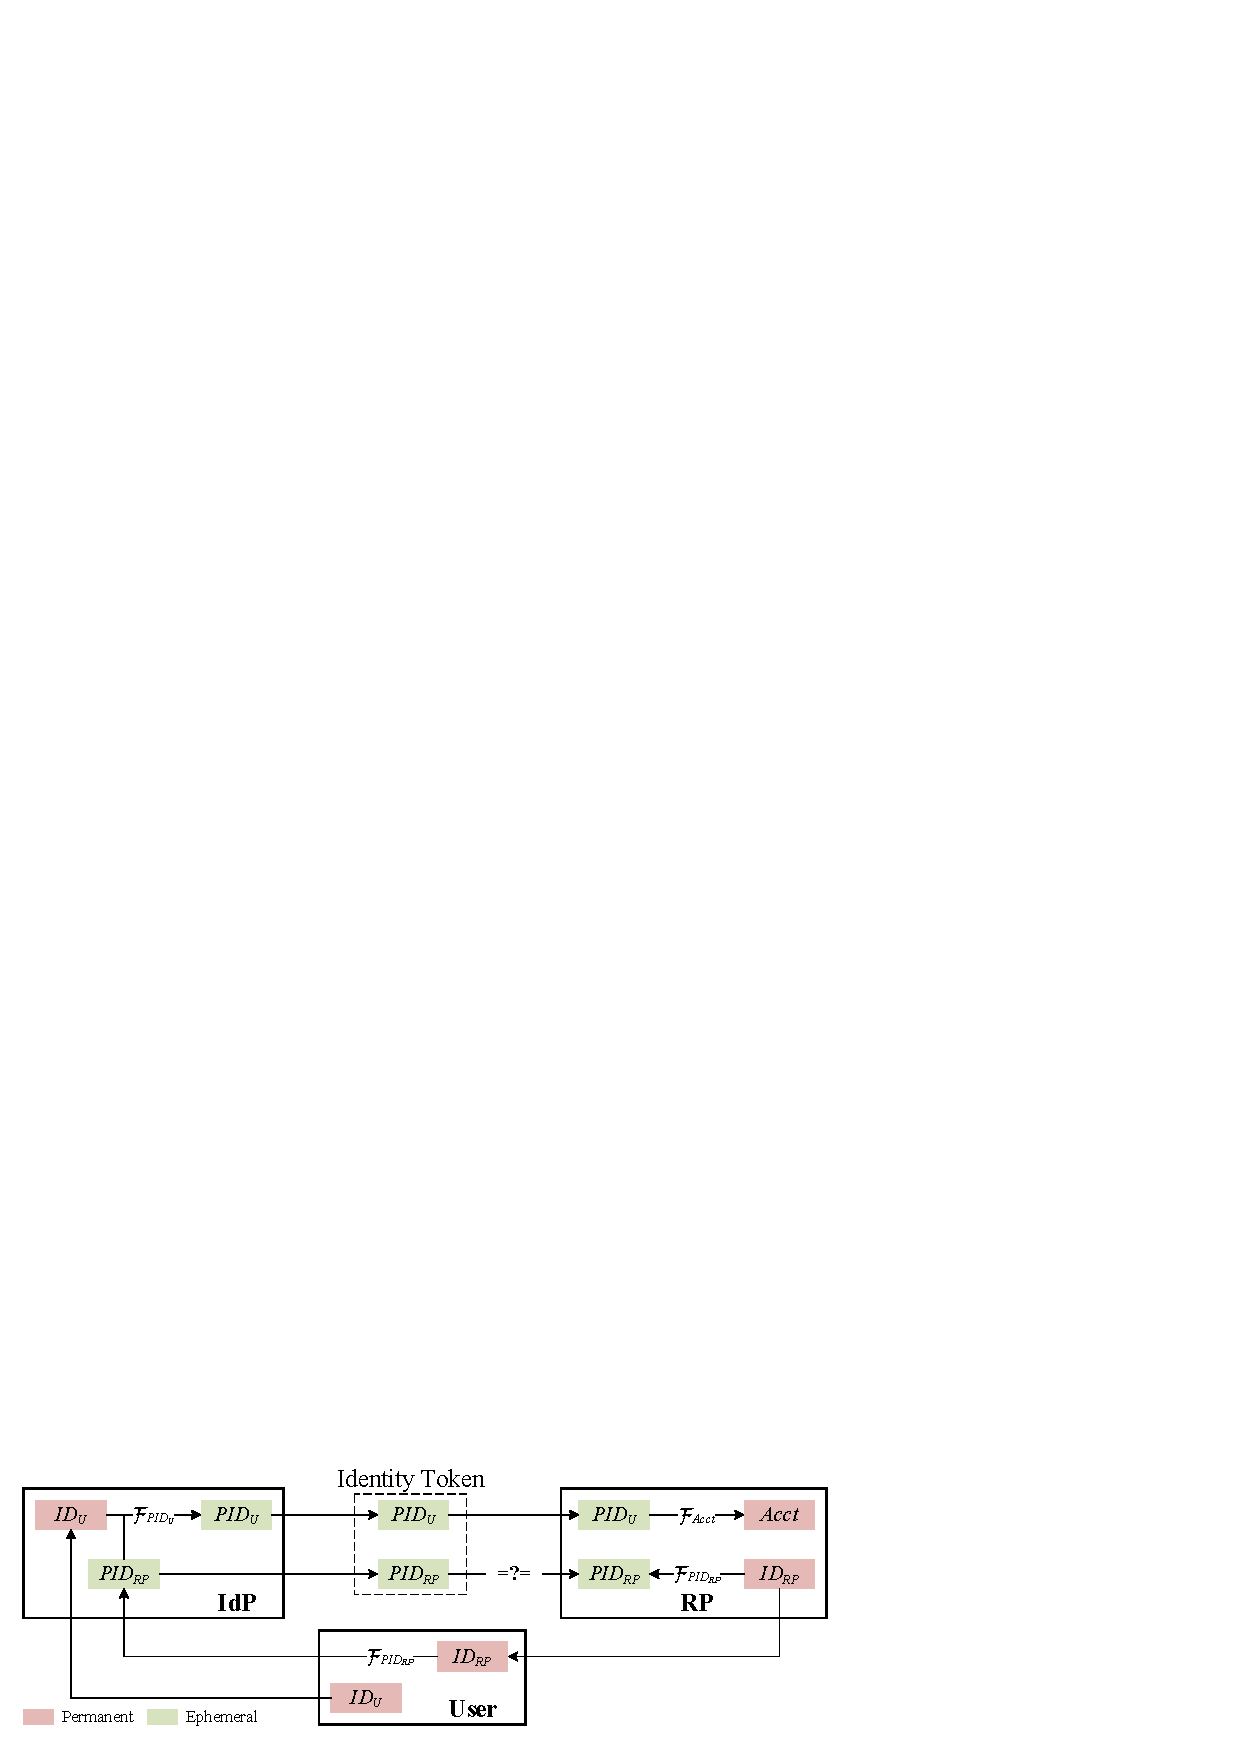
\includegraphics[width=\linewidth]{fig/IDCorrelation.pdf}
  \caption{ID transformations in a privacy-preserving SSO system.}
  \label{fig:IDCorrelation}
\end{figure}

The above analysis demonstrates that the identifers of the user and RP need to be carefully processed in SSO systems.
Here, we systematically analyze the forms of the user and RP identifiers, as required by privacy protection.
As in Figure~\ref{fig:IDCorrelation},
 IdP, who knows the user's globally unique identifer ($ID_U$), should only obtain a privacy-preserving identifer for an RP ($PID_{RP}$);
 each RP, who knows its globally unique identifer ($ID_{RP}$), should only receive a privacy-preserving identifer for a user ($PID_{U}$) from the identity proof.
The $PID_{RP}$ may be null, it means IdP has no information about RP, for example in BrowserID~\cite{BrowserID}.
The $PID_{U}$ can never be null, as RP has to derive the $Accout$ from it, which is the basic function of SSO systems.
Here the  privacy-preserving identifers in multiple sessions will never leak the globally unique identifer nor link the sessions from an entity (the RP and user).
That is, $PID_{RP}$s in multiple login instances for a same RP  should be independent from the view of the IdP;
 and for the collusive RPs, their obtained $PID_{U}$s for a same user should be independent.

Then, we analyze the generation and use of $PID_U$ and $PID_{RP}$, considering the basic requirements of SSO system.
\begin{itemize}
  \item %Who generates $PID_U$? ������IdP��������PID_U
        IdP is the only trusted entity to control the generation of $PID_U$, as the user is not trusted by the RP and a malicious user may provide incorrect $PID_U$. Here, the ``control" means, IdP may generate $PID_U$ alone or with the corporation from the user, but it's the IdP who finally determines the value of $PID_U$. For clarity, we assume IdP generates $PID_U$ by invoking $\mathcal{F}_{ID_{U} \mapsto PID_{U}}$ with $ID_U$ and $PID_{RP}$, without loss of generality.

  \item %What's the requirement considering $PID_{U}$ and $PID_{RP}$ together? $PID_{U}$ and $PID_{RP}$һ����ʱ��Ҫ����ġ�
  The generation of $PID_{U}$ and $PID_{RP}$ must ensure the \textbf{user identification},
  that is, the RP could derive a same $Account$ with the $PID_{U}$ and $PID_{RP}$ from different logins. We assume RP calculates $Account$ by invoking $\mathcal{F}_{PID_{U} \mapsto Account}$ with $PID_U$, $ID_{RP}$ and $PID_{RP}$.

  \item %Who generates $PID_{RP}$, and what's the requirement? PID_RP������RP����user�������ɣ���Ҫ��֤Ψһ�ԡ�
  Each $PID_{RP}$ must be globally unique, i.e., only assigned to one RP,  for achieving the \textbf{receiver designation}.
        The user and RP may generate the $PID_{RP}$ separately or cooperatively, through the function $\mathcal{F}_{ID_{RP} \mapsto PID_{RP}}$.
        However, both the user and RP must check the uniqueness of $PID_{RP}$ before accept and use it.
        If either the user or the RP doesn't perform the check, the adversary could make it accept a $PID_{RP}$ same as an RP and then misuse the identity proof.
        %$PID_{RP}$ is one form of the RP's identifer, and seems unrelated with the user's identifier.
        %Although, the user may inject the user's information into $PID_{RP}$, these information will be treated as random values at the RP and never be used to calculate $Account$, as the user is not trusted by the RP.
        %Therefore, we can assume that $PID_{RP}$ is generated through $\mathcal{F}_{ID_{RP} \mapsto PID_{RP}}$ with the parameter $ID_{RP}$.~\footnote{The $PID_{RP}$ may also be related with the previous $PID_{RP}$. We omit the previous $PID_{RP}$ in the parameters as it is also a transformation of $ID_{RP}$.}
  \item The \textbf{receiver designation} further requires that  $PID_{U}$ is bound with either a non-null $PID_{RP}$ or $ID_{RP}$ in identity proof.
        When $PID_{RP}$  is non-null, IdP builds the identity proof separately and the \textbf{integrity} is also ensured.
        When $PID_{RP}$  is null, only the user cloud bind $PID_{U}$ with an RP identifier (i.e., $ID_{RP}$) which is unique and checkable to the RP.
        In this case, the user who performs the binding, must have a publicly verifiable grant from the IdP, as required by \textbf{integrity}.
        The binding and integrity cloud be achieved by existing public key infrastructure.
   \item The \textbf{receiver designation} also requires the identity proof will only be sent to the correct RP.
       As IdP doesn't know $ID_{RP}$, the user or a third party trusted by the correct RP will ensure this.
\end{itemize}


\subsection{The Principles of UPRESSO}
\label{subsec:solutions}

The dilemma in the design of a secure but privacy-preserving SSO system,
 is solved by finding three privacy-preserving ID transformation functions  $\mathcal{F}_{ID_{RP} \mapsto PID_{RP}}$, $\mathcal{F}_{ID_{U} \mapsto PID_{U}}$,  and $\mathcal{F}_{PID_{U} \mapsto Account}$, which satisfying:
\begin{itemize}
  \item For an RP, $\mathcal{F}_{ID_{RP} \mapsto PID_{RP}}$ generates $PID_{RP}$s in multiple logins, and these  $PID_{RP}$s are independent to the IdP.
  \item For a user, $\mathcal{F}_{ID_{U} \mapsto PID_{U}}$ generates $PID_{U}$s in multiple logins at different RPs, and these $PID_{U}$s are independent to these RPs. $\mathcal{F}_{PID_{U} \mapsto Account}$ outputs $Account$s for a user at different RPs, and these $Account$ are independent to these RPs.
  \item For a user and an RP, $\mathcal{F}_{PID_{U} \mapsto Account}$ generates a unchanged $Account$ in multiple logins.
\end{itemize}

We present UPRESSO, a secure and privacy-preserving SSO system,
which prevents the IdP-based access tracing and RP-based identity linkage under the prerequisites that  the basic requirements of SSO systems are satisfied.
UPRESSO adopts the public key infrastructure to ensure the integrity of the identity proof and TLS for its confidentiality, which is the same as other SSO systems.
Therefore, we focus on how to provide the privacy-preserving user identification and receiver designation as follows:

\vspace{1mm}\noindent \textbf{Trapdoor user identification.} UPRESSO breaks the implicit assumption in previous SSO systems, that an RP should obtain an unchanged value to identify a user in the multiple logins.
A trapdoor identification is introduced, which allows the RP  to derive the unchanged $Accout$ from different $PID_{U}$s.
The trapdoor identification requires a cooperation of the three functions $\mathcal{F}_{ID_{RP} \mapsto PID_{RP}}$, $\mathcal{F}_{ID_{U} \mapsto PID_{U}}$ and $\mathcal{F}_{PID_{U} \mapsto Account}$.
$\mathcal{F}_{ID_{RP} \mapsto PID_{RP}}$  is invoked with a trapdoor to generate $PID_{RP}s$ which are independent to IdP (preventing IdP-based access tracing),
 and RP uses $\mathcal{F}_{PID_{U} \mapsto Account}$ with this trapdoor to derive the unchanged $Accout$  from $PID_{U}$s that are generated by IdP with $\mathcal{F}_{ID_{U} \mapsto PID_{U}}$.

\vspace{1mm}\noindent \textbf{Transformed receiver designation.}
UPRESSO splits the receiver designation into two steps: IdP designates the identity proof to a transformed RP identifer (i.e., $PID_{RP}$), while the user and RP cooperatively designate a fresh and unique $PID_{RP}$ only to one $ID_{RP}$. Then, each RP only needs to check the designation based on $PID_{RP}$.
\begin{itemize}
  \item In the first step, the IdP generates $PID_U$ for $PID_{RP}$ and achieves full privacy-preserving binding (i.e., $PID_U$ with $PID_{RP}$).
UPRESSO introduces an efficient one-way (trapdoor) function $\mathcal{F}_{ID_{U} \mapsto PID_{U}}$.
 It allows IdP to  compute $PID_U$ easily,  avoiding the generation of $PID_U$ to be the bottleneck at a high-throughput IdP;
   and also prevents the RP from finding any information about $ID_U$, which is required by preventing RP-based identity linkage.
  \item In the second step, the user and RP cooperatively generate a fresh $PID_{RP}$ based on $\mathcal{F}_{ID_{RP} \mapsto PID_{RP}}$ and check the uniqueness of the $PID_{RP}$, therefore a fresh and unique $PID_{RP}$ is only mapped to one RP, when at least a correct user or correct RP exists. Moreover, the user needs to extract the correct endpoint of $ID_{RP}$, to ensure that the  identity proof is sent to the only correct RP.
\end{itemize}

To meet the above two principles, we need to construct three satisfying functions $\mathcal{F}_{ID_{RP} \mapsto PID_{RP}}$, $\mathcal{F}_{ID_{U} \mapsto PID_{U}}$ and $\mathcal{F}_{PID_{U} \mapsto Account}$, design the protocols between the user, RP and IdP to avoid the privacy leakage during message transmission, and implement the  processing at the user as  required by the transformed receiver designation.


\subsection{Existing Solutions}
Various solutions~\cite{OpenIDConnect, SAMLIdentifier,BrowserID,SPRESSO}, are proposed, attempting to construct a secure and privacy-preserving SSO system.
However, these scheme provide at most two satisfying functions, and therefore fail to prevent either the IdP-based access tracing or RP-based identity linkage.
\begin{itemize}
  \item The traditional SSO systems provide no satisfying functions, and therefore fail to protect the user's privacy.
  \item SAML~\cite{SAMLIdentifier} and OIDC~\cite{OpenIDConnect} provide only the satisfying $\mathcal{F}_{ID_{U} \mapsto PID_{U}}$ and $\mathcal{F}_{PID_{U} \mapsto Account}$ .
        The IdP obtains the $ID_{RP}$ for an RP, and generates the unchanged $PID_{U}$ for the same couple $<ID_{U}$, $ID_{RP}>$,
        while the $PID_{U}$ are independent for different $ID_{RP}$s.
  \item BrowserID~\cite{BrowserID} and SPRESSO~\cite{SPRESSO} provide only the satisfying $\mathcal{F}_{ID_{RP} \mapsto PID_{RP}}$.
        In BrowserID, IdP obtains a null $PID_{RP}$ and provides $ID_U$ to the RP, therefore each RP obtains the unchanged $Accout$.
        In SPRESSO, each RP generates $PID_{RP}$ by encrypting $ID_{RP}$ padding by a random nonce,
        and IdP provides the unchanged $ID_U$ for a user's multiple logins no matter which RP the user is visiting.
\end{itemize}

Obliviously, existing attempts fail to provide the complete  privacy.
The essential reason is that these schemes provide an unchanged value (e.g., $PID_{U}$ in SAML~\cite{SAMLIdentifier} and OIDC~\cite{OpenIDConnect}, or $ID_U$ in BrowserID~\cite{BrowserID} and SPRESSO~\cite{SPRESSO}) for the user's multiple logins at an RP.
To provide unchanged $PID_{U}$, IdP has to know $ID_{RP}$ and then will be able to identity or link the logins at an RP.
Providing $ID_U$ to the RP, makes  the collusive RPs easily link the user's logins at different RPs.

